As early as 2001, researchers have proposed the use of a novel, hybrid engine
design for use in supersonic and hypersonic flight \cite{Macheret2001}. In some
ways similar to an earlier program \cite{Gurijanov1996}, it suggested that
magnetohydrodynamic (\acs{mhd}) accelerators were an enabling technology for
hypersonic transport. Briefly, a \acs{mhd} accelerator could be used to
simultaneously produce energy and slow the inlet airflow. This would allow the
use of a conventional turbojet engine at speeds well above its normal
operational range.

However, \acs{mhd} accelerators require an ionized fluid flow. Even at the high
altitudes associated with hypersonic flight, this is not easy to achieve.
Originally, Macheret suggested the use of electron beams, carefully tuned to
coincide with the peak in the ionization cross section in air. However, the use
of electron beams in the ionization of high pressure gases is accompanied by a
large number of technical issues, similar to those of some excimer lasers.
Therefore, in 2002, Macheret et al.\ proposed the use of a \acs{rpnd} to produce
an ``electron beam'' in situ \cite{Macheret2002} akin to the beams observed in
certain \acs{fiw} studies.

The use of a \acs{rpnd} is accompanied by a reduced ionization efficiency in
comparison to an electron beam. However, it reduces the some of the
implementation challenges and Macheret argued that it offered a more efficient
and stable option than breakdown with DC electric fields. Though the densities
of \acs{fiw}s in several air-related chemistries have been measured on several
occassions \cite{Anikin1998, Aleksandrov2007, Aleksandrov2008,
Starikovskaia2006}, similar studies do not appear to exist for \acs{rpnd}s in
air. Therefore, there is a need for electron density measurements to confirm
that \acs{rpnd}s are adequate for the \acs{mhd} accelerator requirements and to
quantify their ionization efficiency.

In addition, previous studies of \acs{fiw}s in air have observed fast gas
heating of molecular systems \cite{Popov2011}. Up to 40\% of the input energy
can be converted into translational energy through dissociation of oxygen and
quenching or electronically excited nitrogen states. As the \acs{rpnd} physics
are very similar to that of the \acs{fiw}, there is the possibility that it may
also cause fast gas heating. In combustion, this can play an important role in
the chemistry, flame holding, and ignition delay. More generally, gas heating
can impact material processing and ionization efficiency. As such, it is
important to develop reliable temperature diagnostics for \acs{rpnd}s in
molecular gases.

This appendix records the development of two diagnostics for an air \acs{rpnd}
at NASA Glenn Research Center. Measurement of the density was accomplished using
millimeter-wave interferometry. Plasma interferometry measures changes in the
phase and amplitude of an electromagnetic wave which has passed through the
plasma \cite{Lieberman2005}. The phase shift is proportional to the density of
electrons while the change in amplitude is related to the electron-neutral
collision frequency. As with other wave-based techniques, the density resulting
from this approach is line integrated. The translational temperature of the
system was measured via 

The light emissions of the second positive system of nitrogen were carefully
modeled and measured in the \textsc{rpnd}. This resulted in time-resolved values
of the rotational and kinetic temperatures of the system.

 of such a diagnostic for a moderate
pressure \acs{rpnd} in air. The approach used measured the rotational spectra of
a molecular system and used this information to infer the rotational
temperature. As a result of the close energy-spacing of the rotational levels,
this temperature is usually a good measure of the translational temperature of
the system \cite{Laux1993}. This technique is limited by the ability to detect
light from the transitions, and by the equilibration time of the translational
and rotational temperatures.

The measurement of rotational transitions is a common diagnostic for the
measurement of gas temperatures, particularly in the field of combustion.
Matching of the rotational spectra is typically accomplished with a computer
program such as Specair \cite{Laux2002} and LIFBASE \cite{Luque1999}. However, a
survey of the available programs revealed little documentation about the
calculation methods and none which provided the necessary flexibility how the
spectra were generated. This necessitated the development of a program to
automate the generation and matching of rotational spectra.

\section{Experiment}

All experiments were conducted in a vacuum chamber at \textsc{nasa grc}. Before
operation, the vacuum chamber was evacuated to the desired pressure
(approximately 20 Torr in all presented cases). After the desired pressure was
reached, the chamber was valved off. As a result, the pressure was subject to
some variation in each of the experiments. When the discharge was initiated for
the first time after a pump down, the chamber pressure would rise by
approximately 2 Torr after several minutes of operation. Afterward, the pressure
would continue to increase at a greatly reduced rate, on the order of several
tenths of a Torr per minute.

The discharge was sustained by two parallel cylindrical electrodes, 2.5 cm in
diameter and 0.625 cm in length. For the interferometry experiment, the
electrodes were mounted in dielectric epoxy cast such that it was flush with the
electrode faces. This was later replaced by a Mykroy fitting, seen in
figure~\ref{fig:electrodes}, for the optical emission experiment. This change
was made to increase the durability of the apparatus for longer experimental
operation.
\begin{figure}
  \centering
  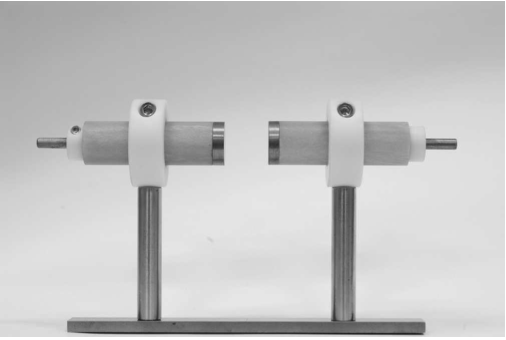
\includegraphics{./chapters/nasa/figures/electrodes.pdf}
  \caption{The electrodes used in the \textsc{pnd} at \textsc{nasa grc}. The
    electrodes are made of copper with a ceramic sheath made of
    Mykroy.}
  \label{fig:electrodes}
\end{figure}
The power supply was built by FID (model FPG 60-100-MC4-S5) and supplied voltage
pulses of up to 60 kV at repetition rates from 6-100 kHz with pulsewidths of 5
ns. Unless otherwise stated, all measurements were made with the power supply
operating at 20 kHz using a Wavetek FG3C as the master clock.
